\begin{recipe}
[ %
	preparationtime = {\SI{1}{\hour}},
	bakingtime={\SIrange{30}{35}{\minute}},
	bakingtemperature={\protect\bakingtemperature{topbottomheat=\SI{350}{\fahrenheit} (\SI{180}{\celsius})}},
%	portion = {\portion[Item]{1}},
	source = {BrainStew}
    ]{Stuffed Mushrooms}

	\begin{figure}[p]
		\centering
		\makebox[\textwidth][c]{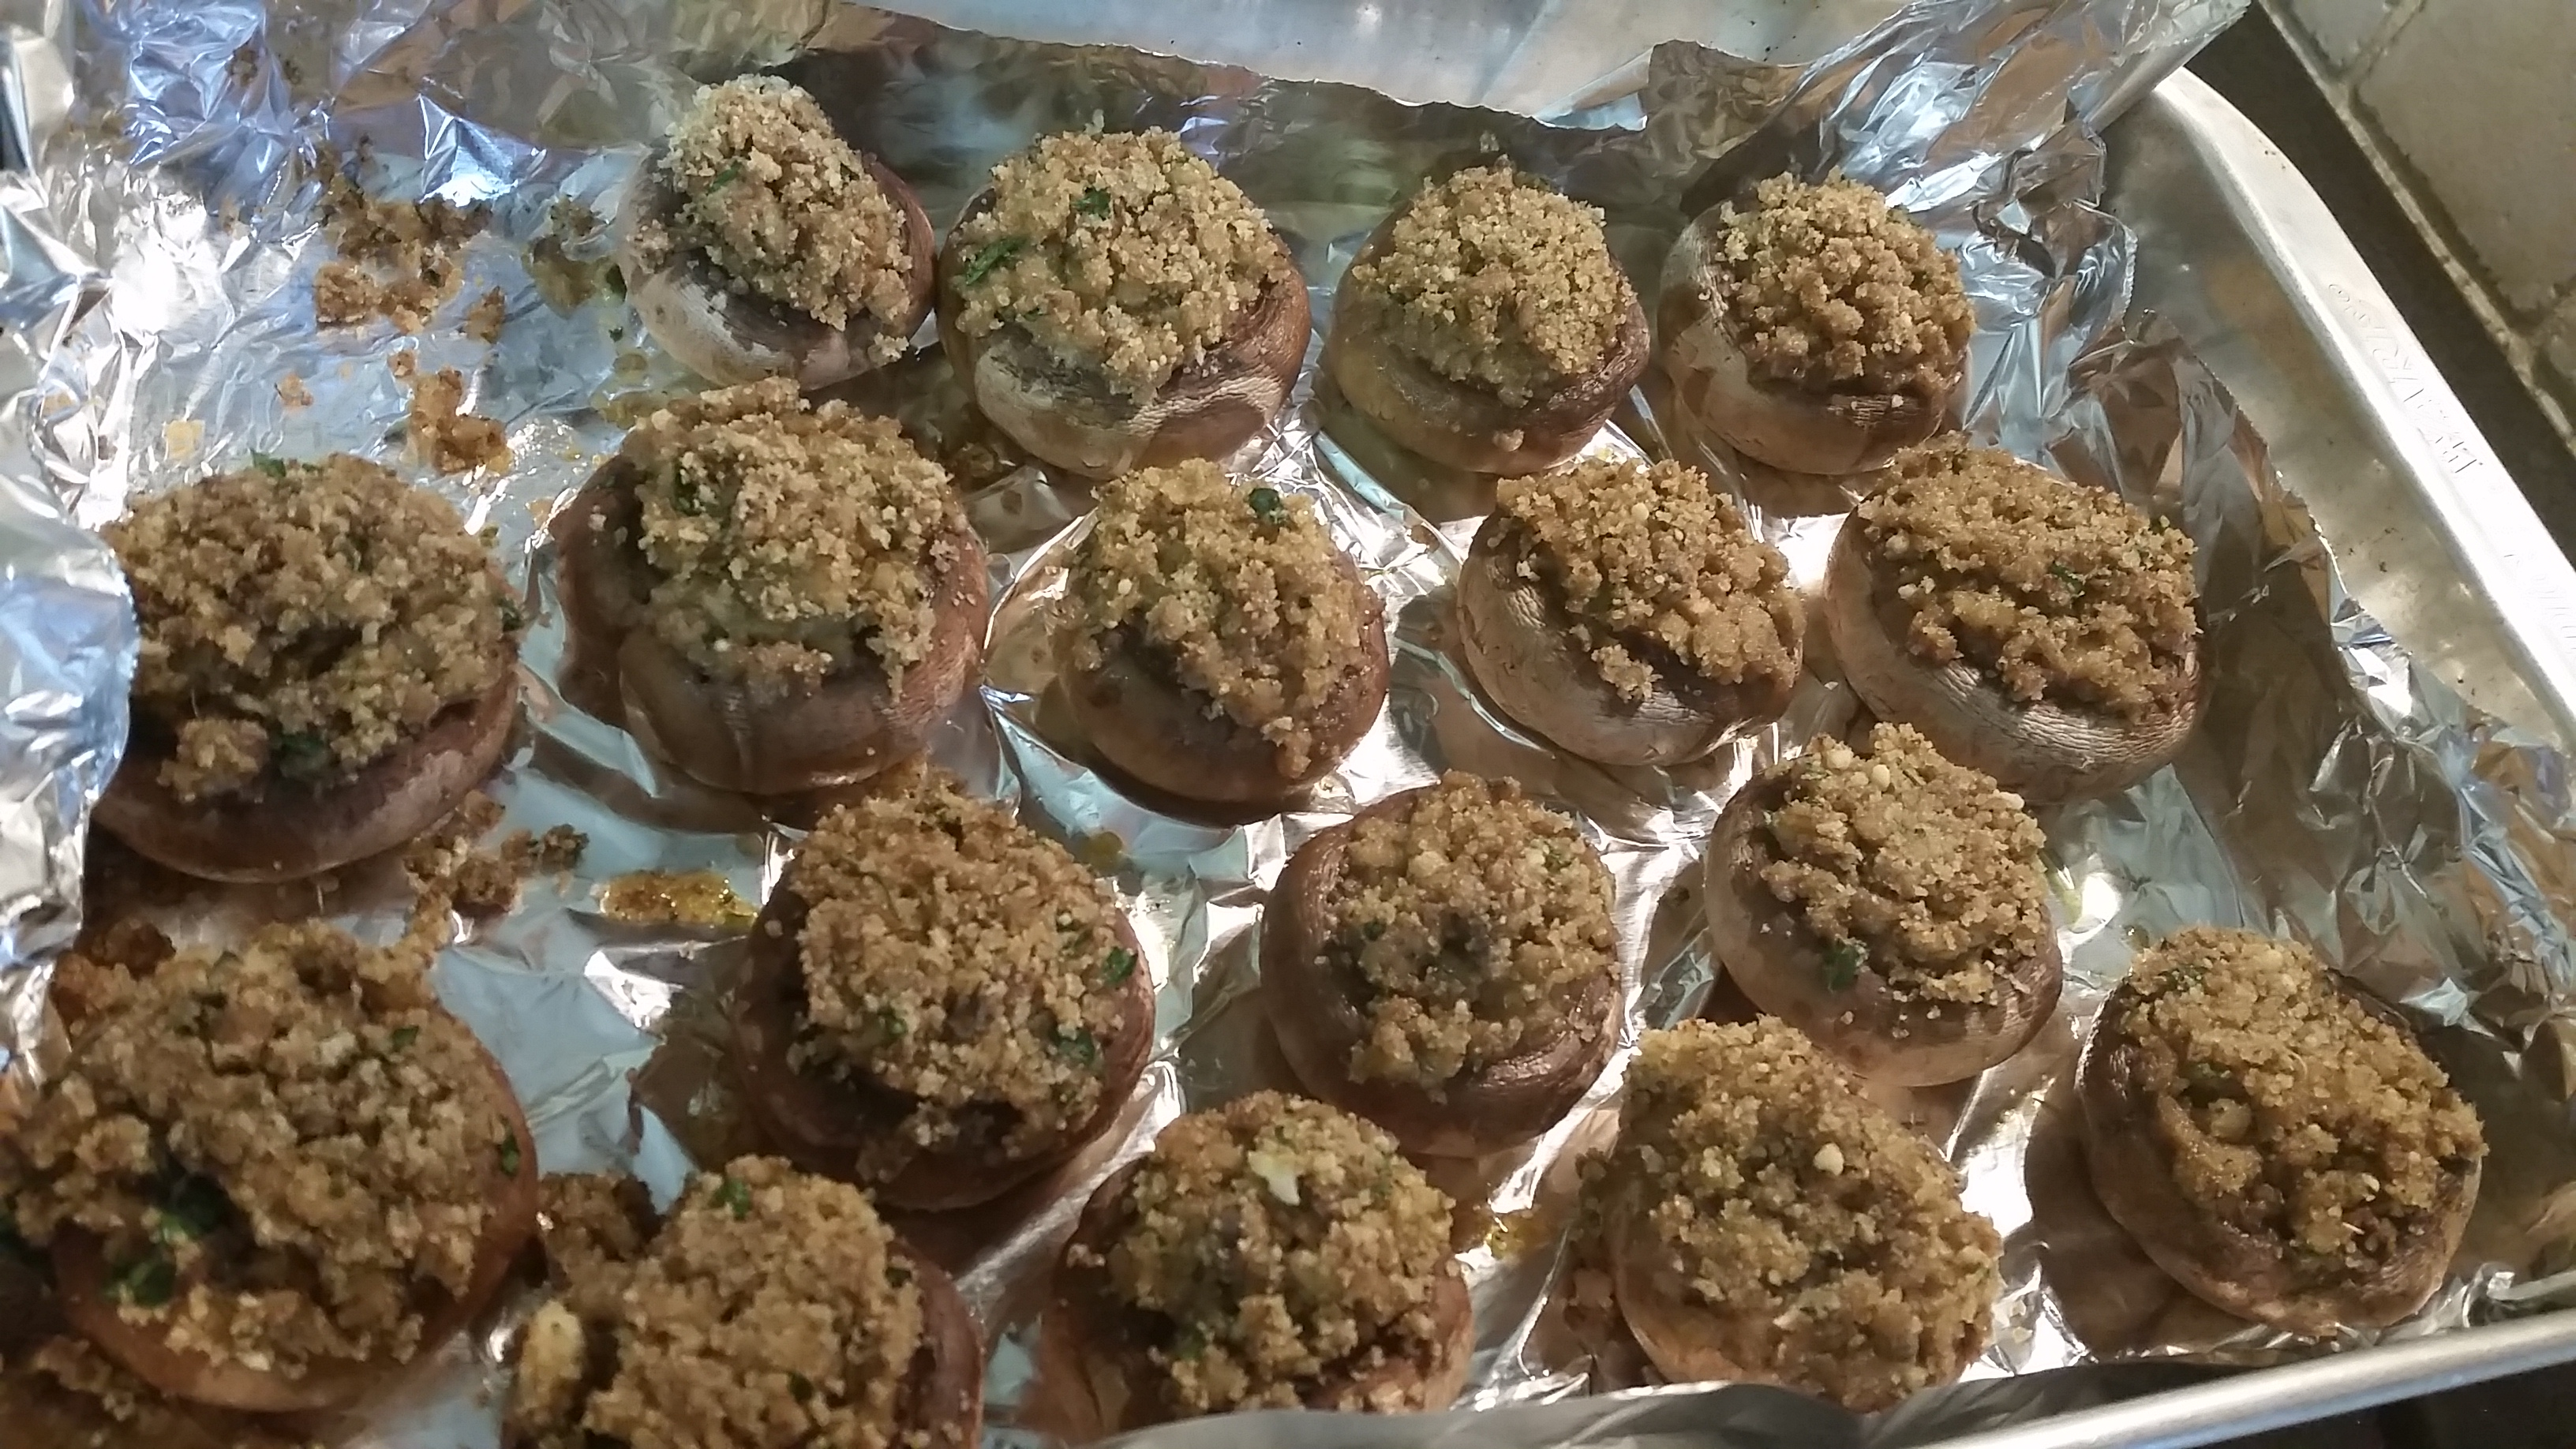
\includegraphics[height=\textheight]{stuffed_mushrooms/20150728_154326.jpg}}
	\end{figure}

    \introduction{
    	Since this is a family recipe, the balance of ingredients depends on the taste of the person making them. This is how I like them, but more or less cheese, parsley, or garlic would not go amiss if you feel any of those things are not to your taste. Since the stuffing is made and fully cooked before it is put into the caps, taste it often to make sure it is to your liking.

    	Also, I used rather large mushrooms in the pictures for this recipe (sometimes called stuffing mushrooms) but usually I use smaller button mushrooms so that more people can have a taste of them. Either is fine, but the cooking time will be less for smaller mushrooms.
	}

	\ingredients[7]{
		\SI{48}{\ounce} & Mushrooms, rubbed clean with a damp paper towel \\
		\SIrange{6}{9}{\tablespoon} & Olive oil \\
		\SIrange{6}{7}{cloves} & Garlic, minced \\
		\SI{1}{\cup} & Italian seasoned bread crumbs, plus more for balancing \\
		\SI{1/3}{\cup} & Grated parmigiano reggiano cheese \\
		\SI{1}{\tablespoon} & Fresh parsley, finely chopped \\
		& Salt and Pepper to taste
	}

	\preparation{
		\step After cleaning the mushrooms, pull the stems out from the caps carefully with a light twisting motion as to not split the caps. If you split a cap and it can still hold stuffing, keep it, otherwise throw it in with the stems. Set the caps aside and gather the stems.

		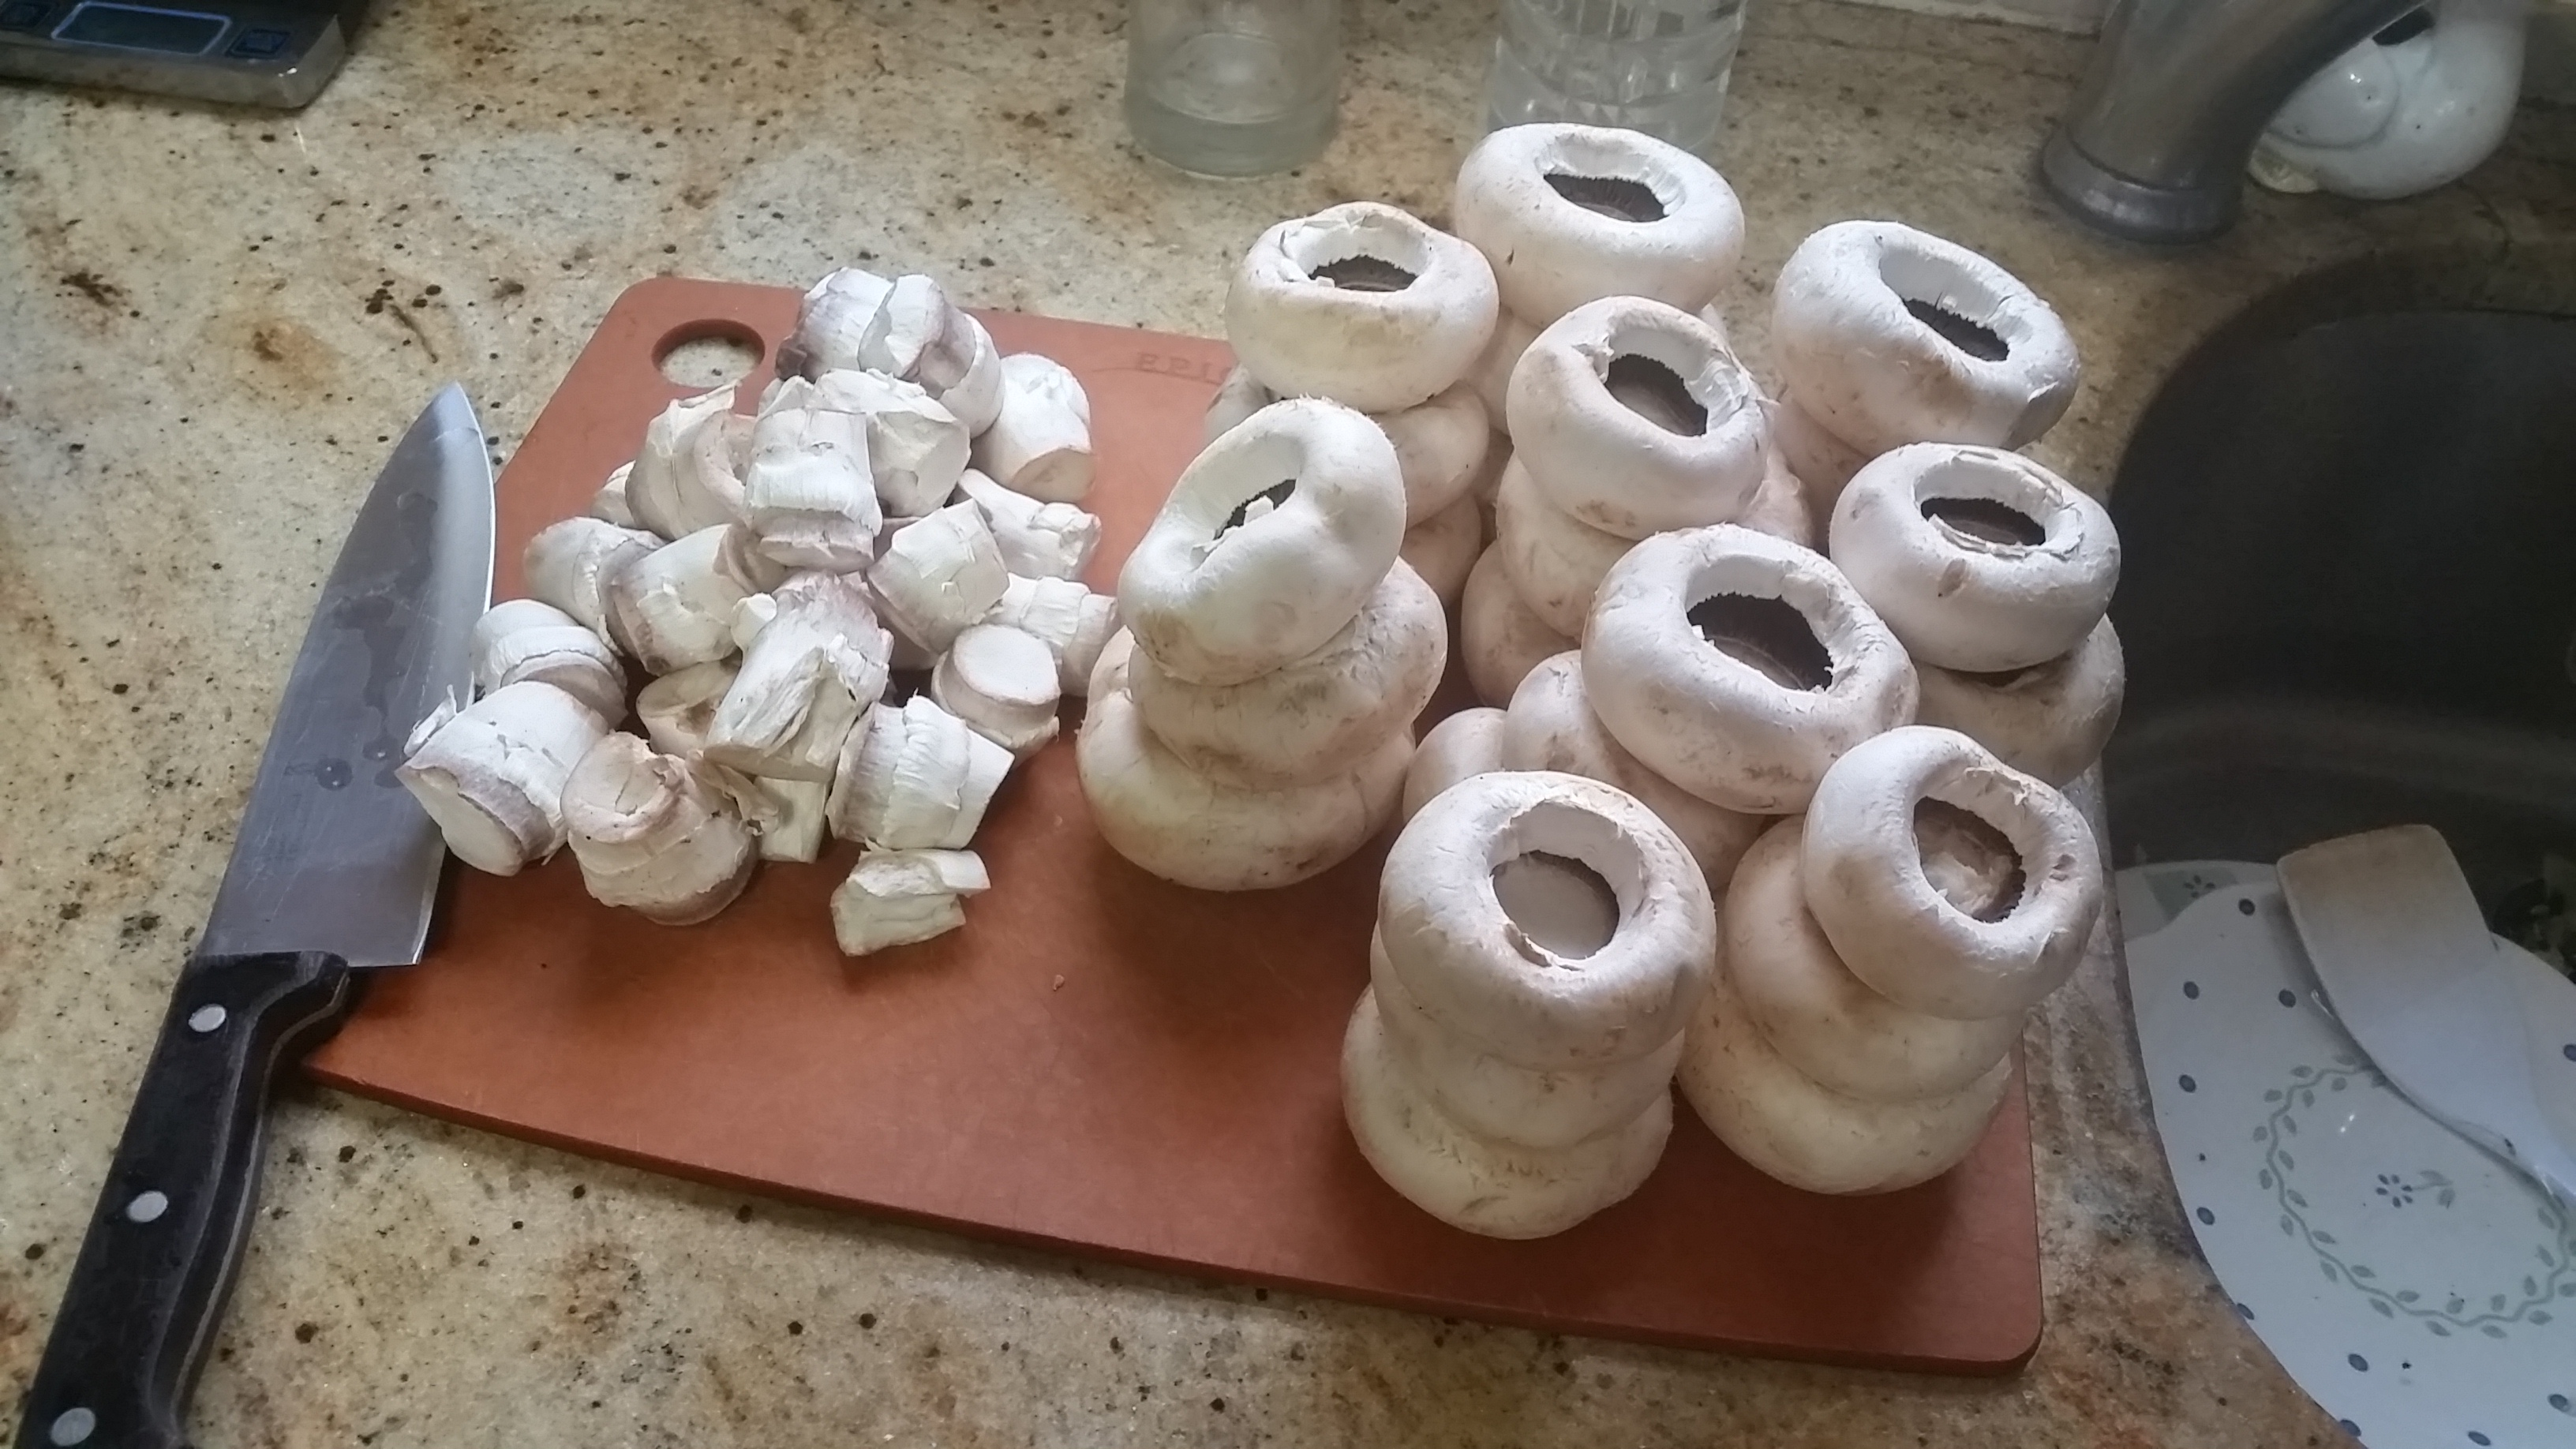
\includegraphics[width=0.52\textwidth]{stuffed_mushrooms/20150728_134346.jpg}

		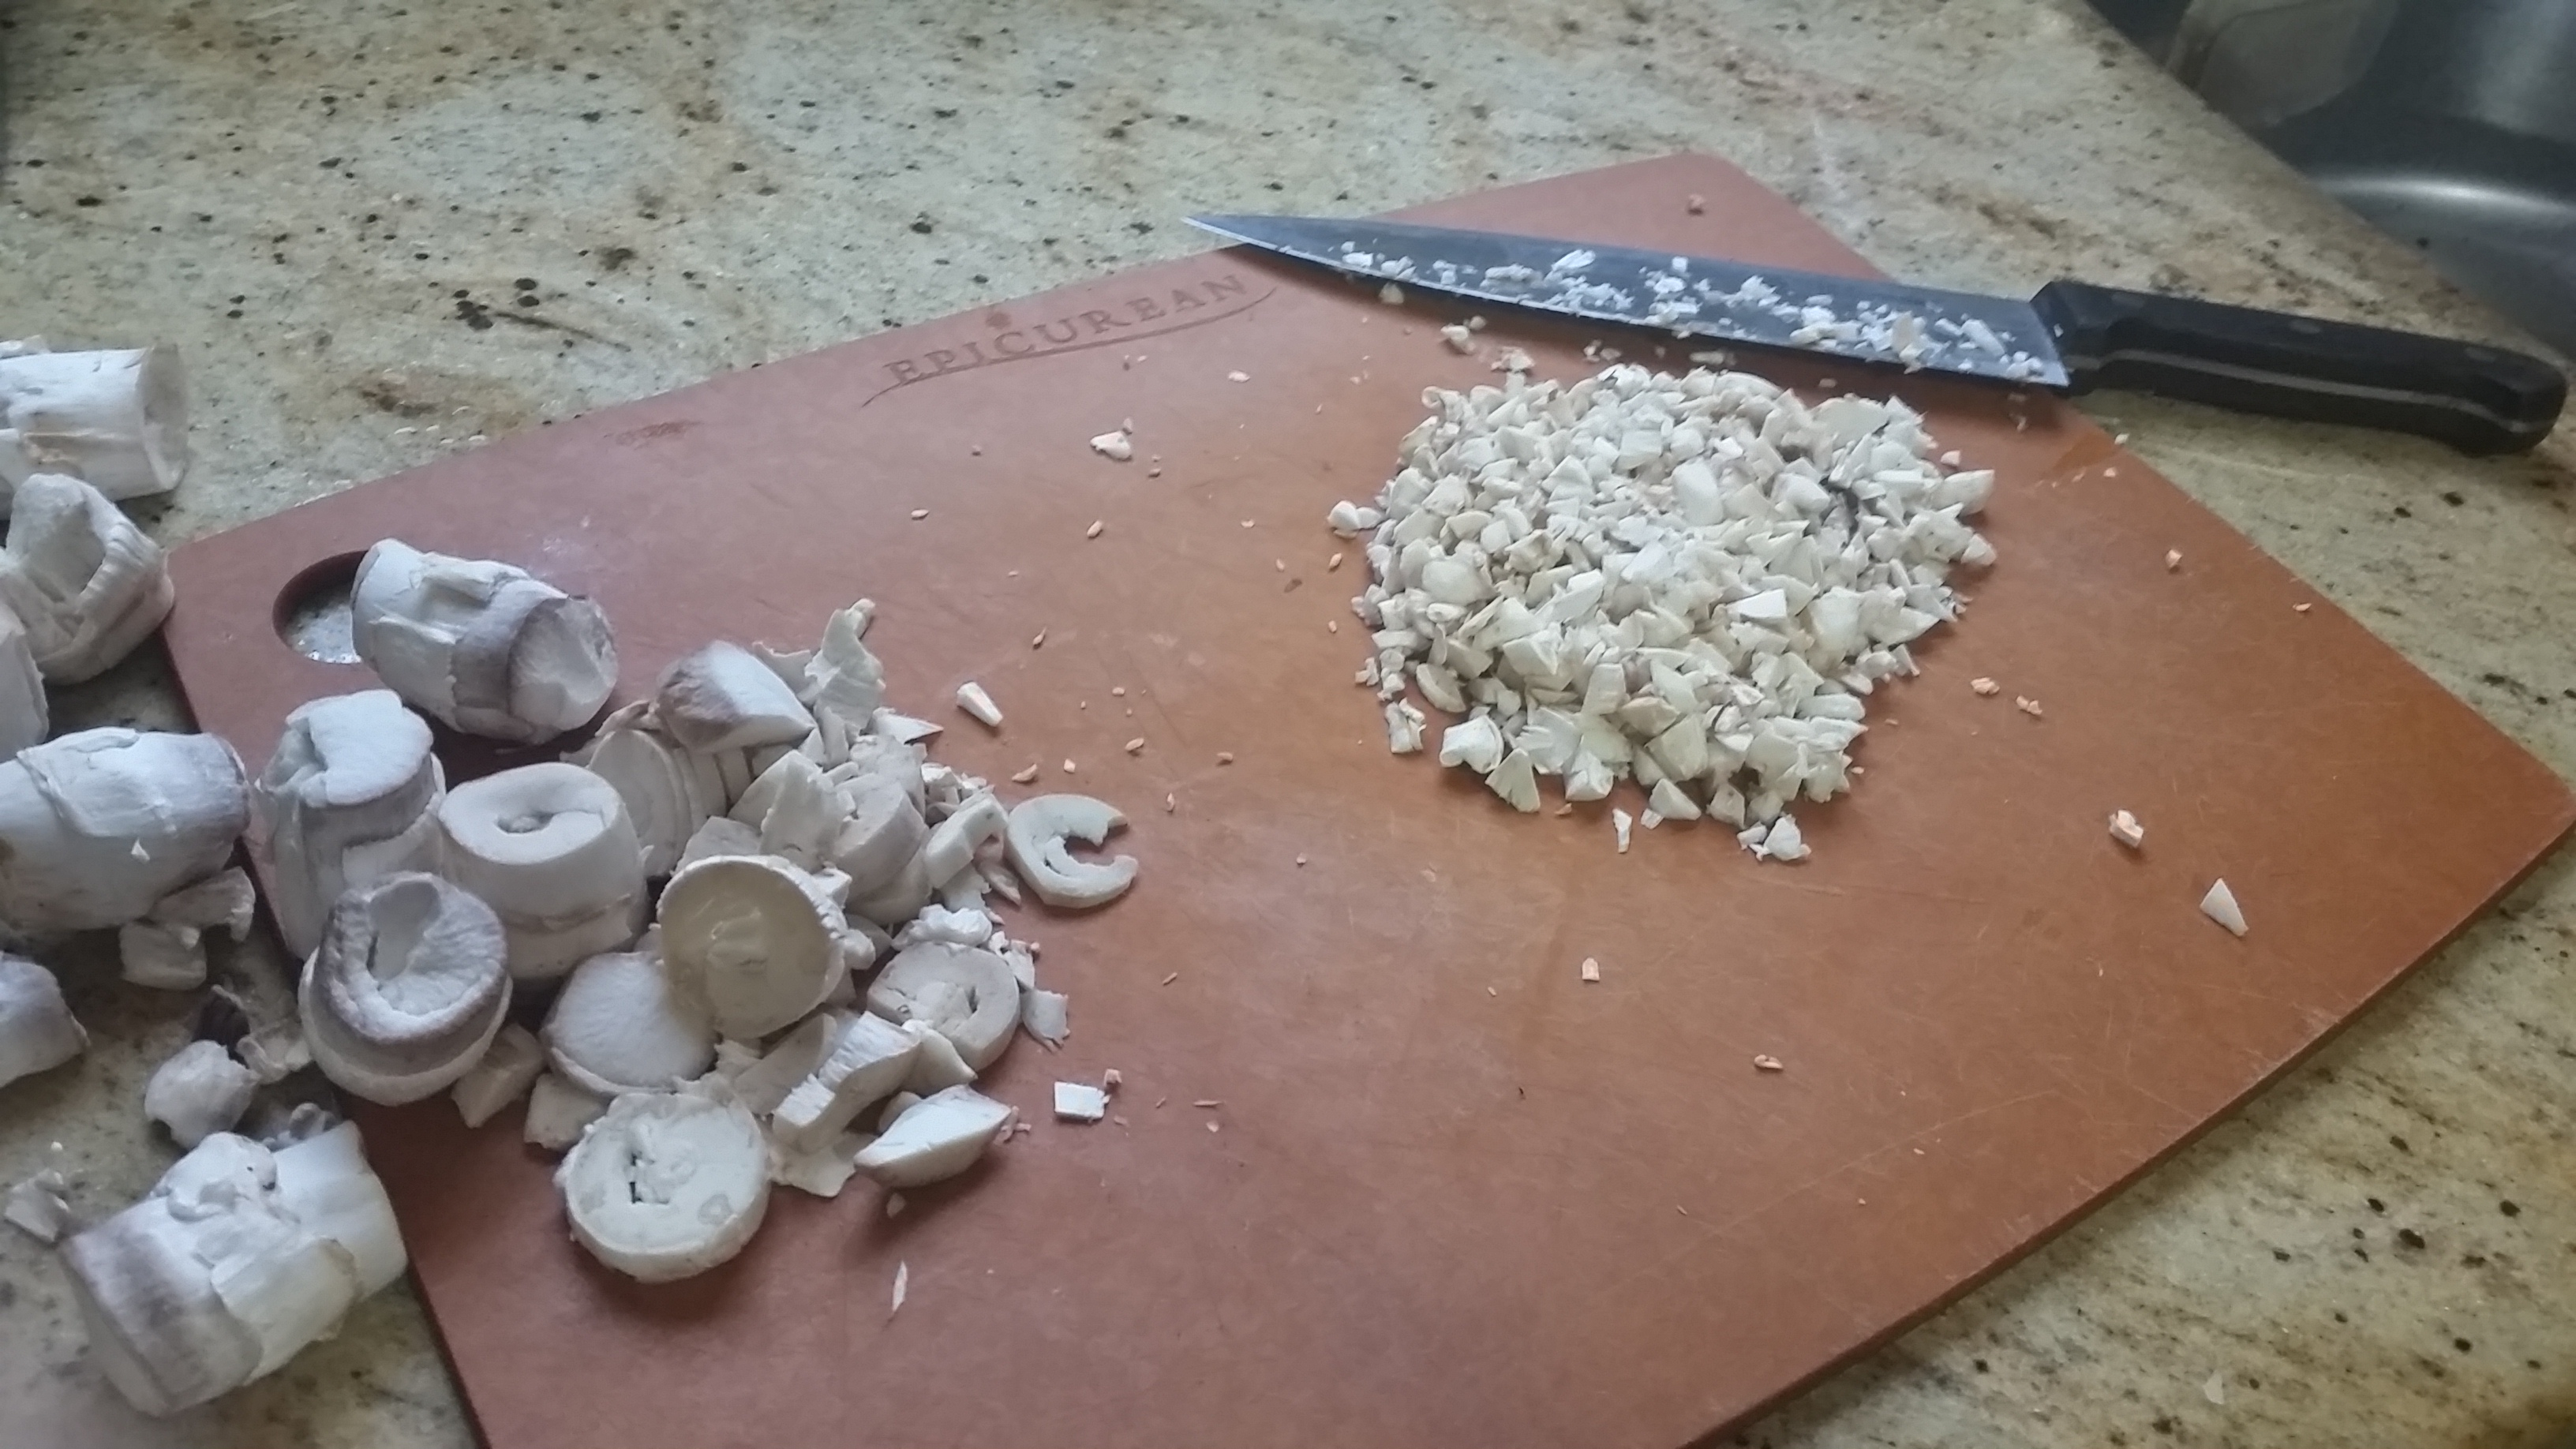
\includegraphics[width=0.5\textwidth]{stuffed_mushrooms/20150728_135626.jpg}%
		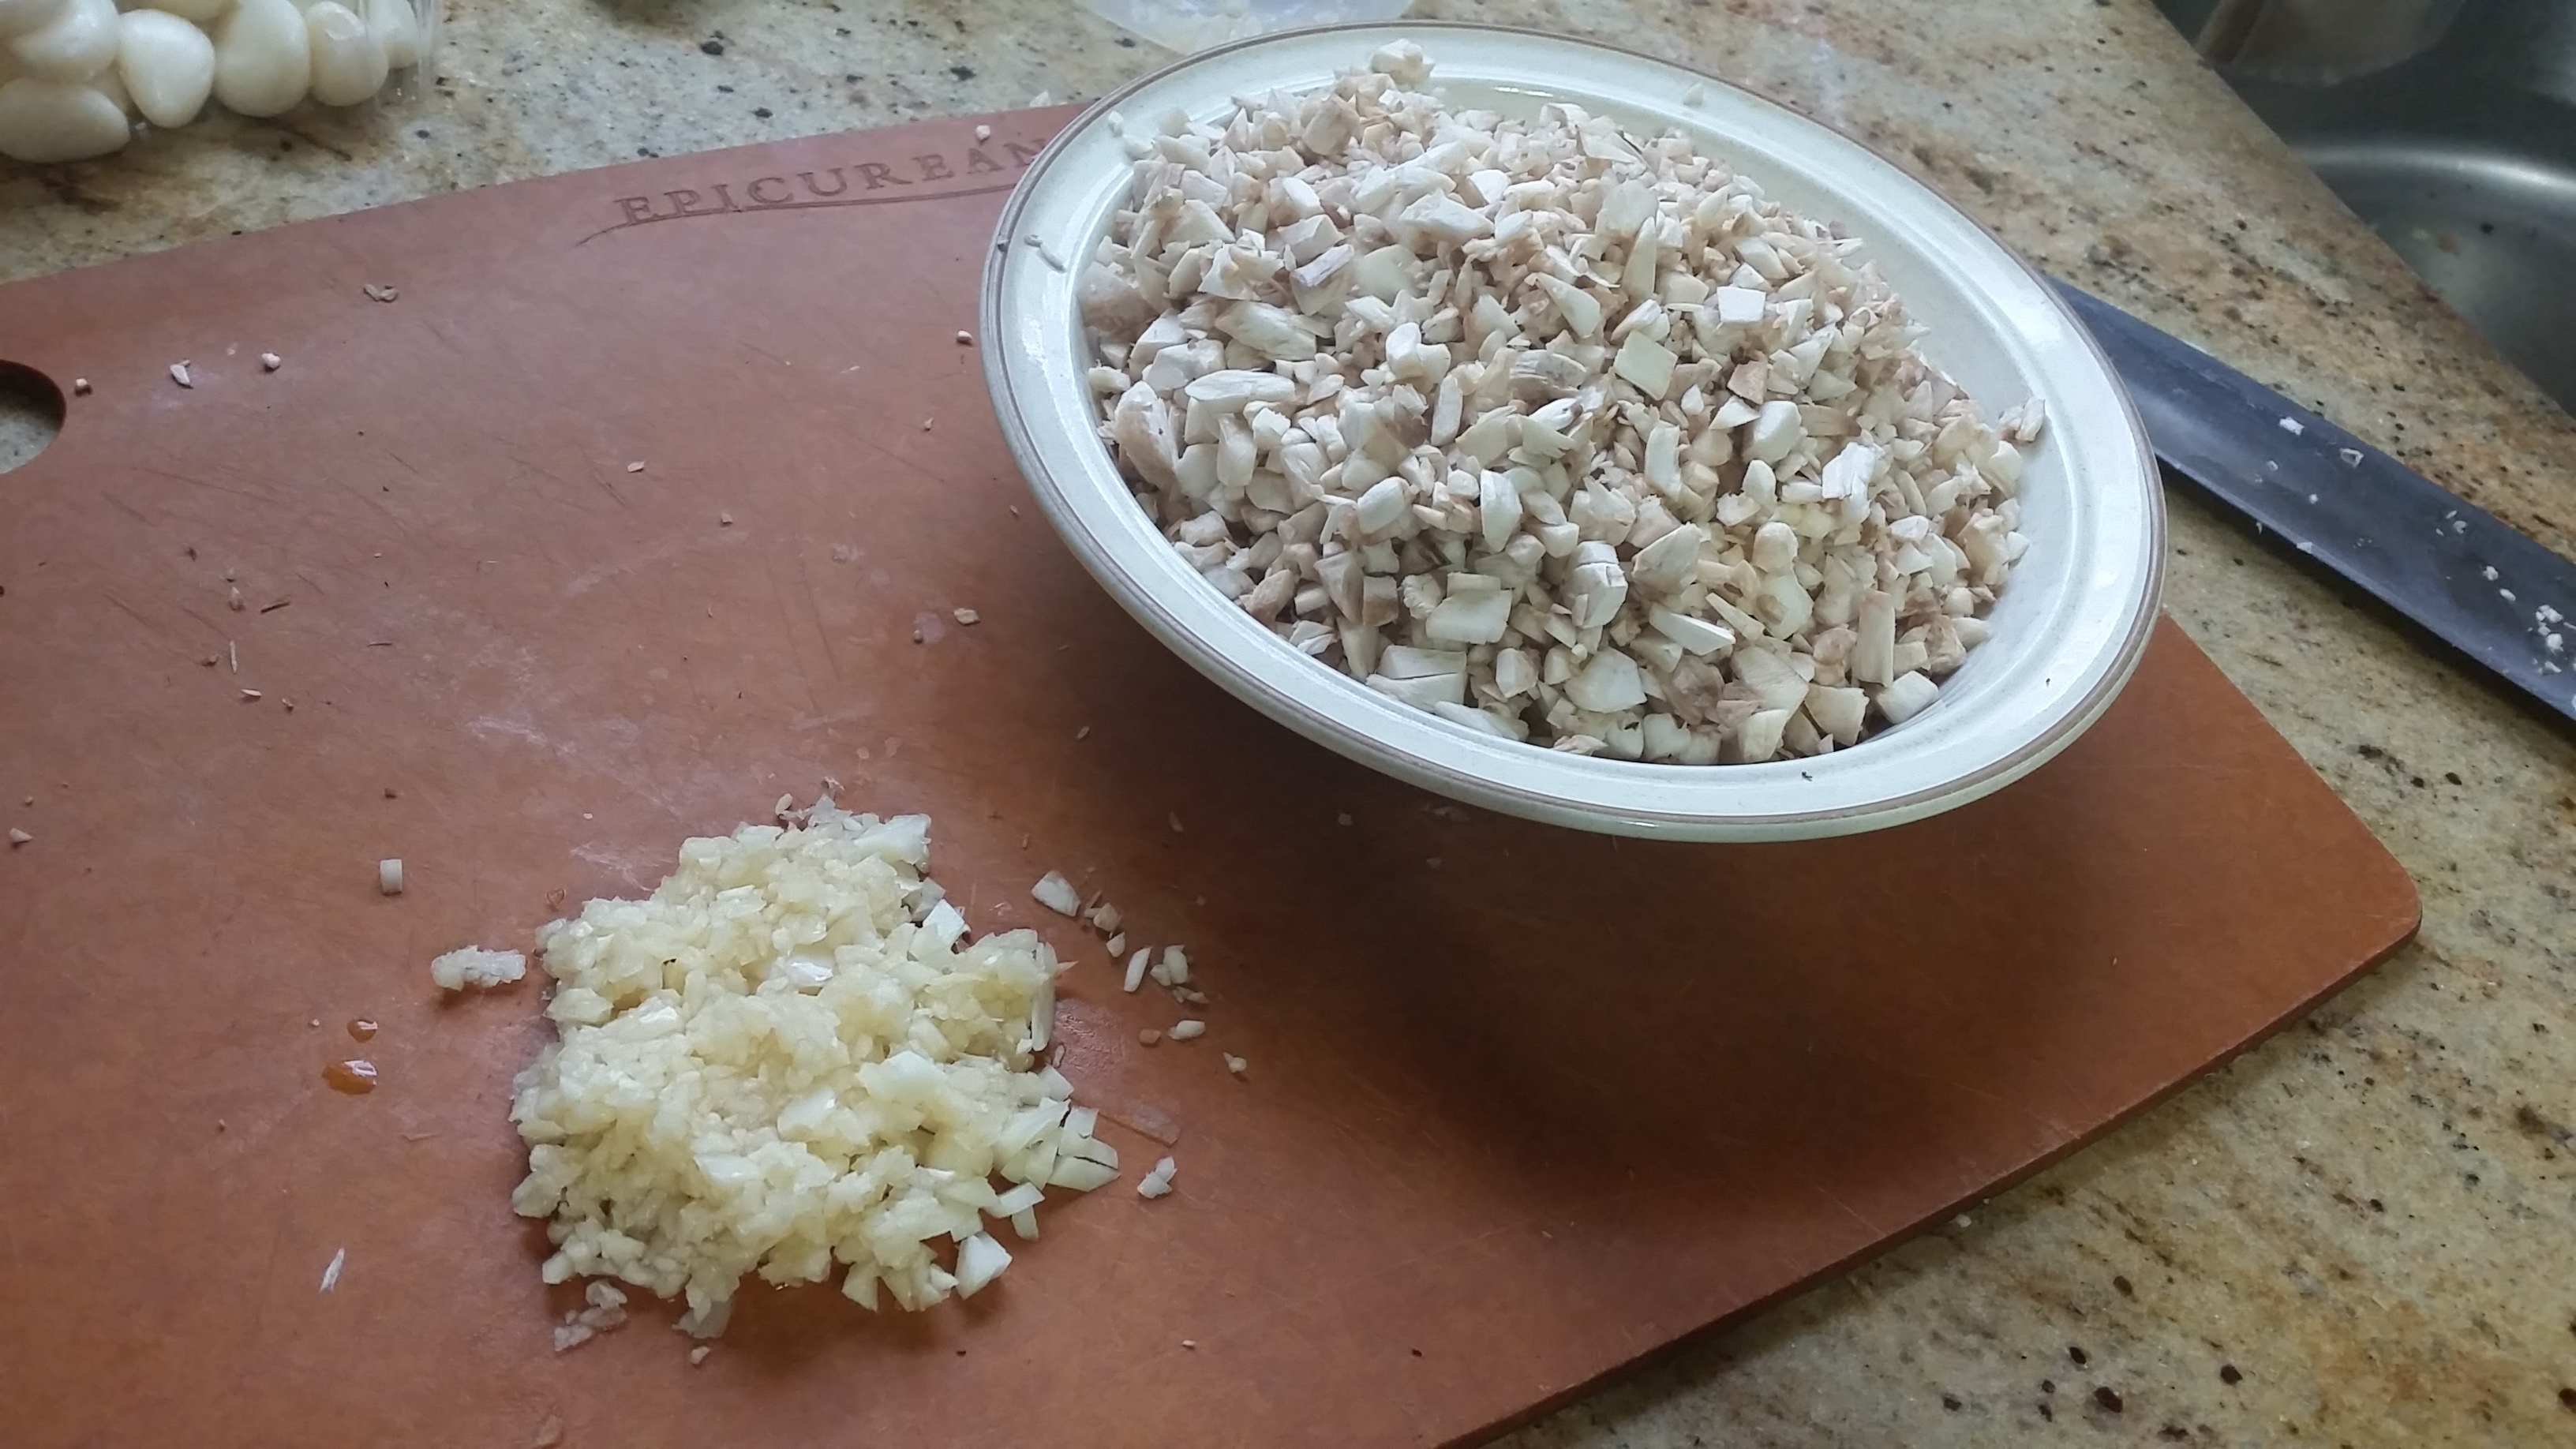
\includegraphics[width=0.5\textwidth]{stuffed_mushrooms/20150728_142451.jpg}

		\step Mince the stems finely as they will be more than half of the stuffing and you don’t want it to be too chunky.

		\step Mince the garlic and parsley as well.

		\vspace{1em}

		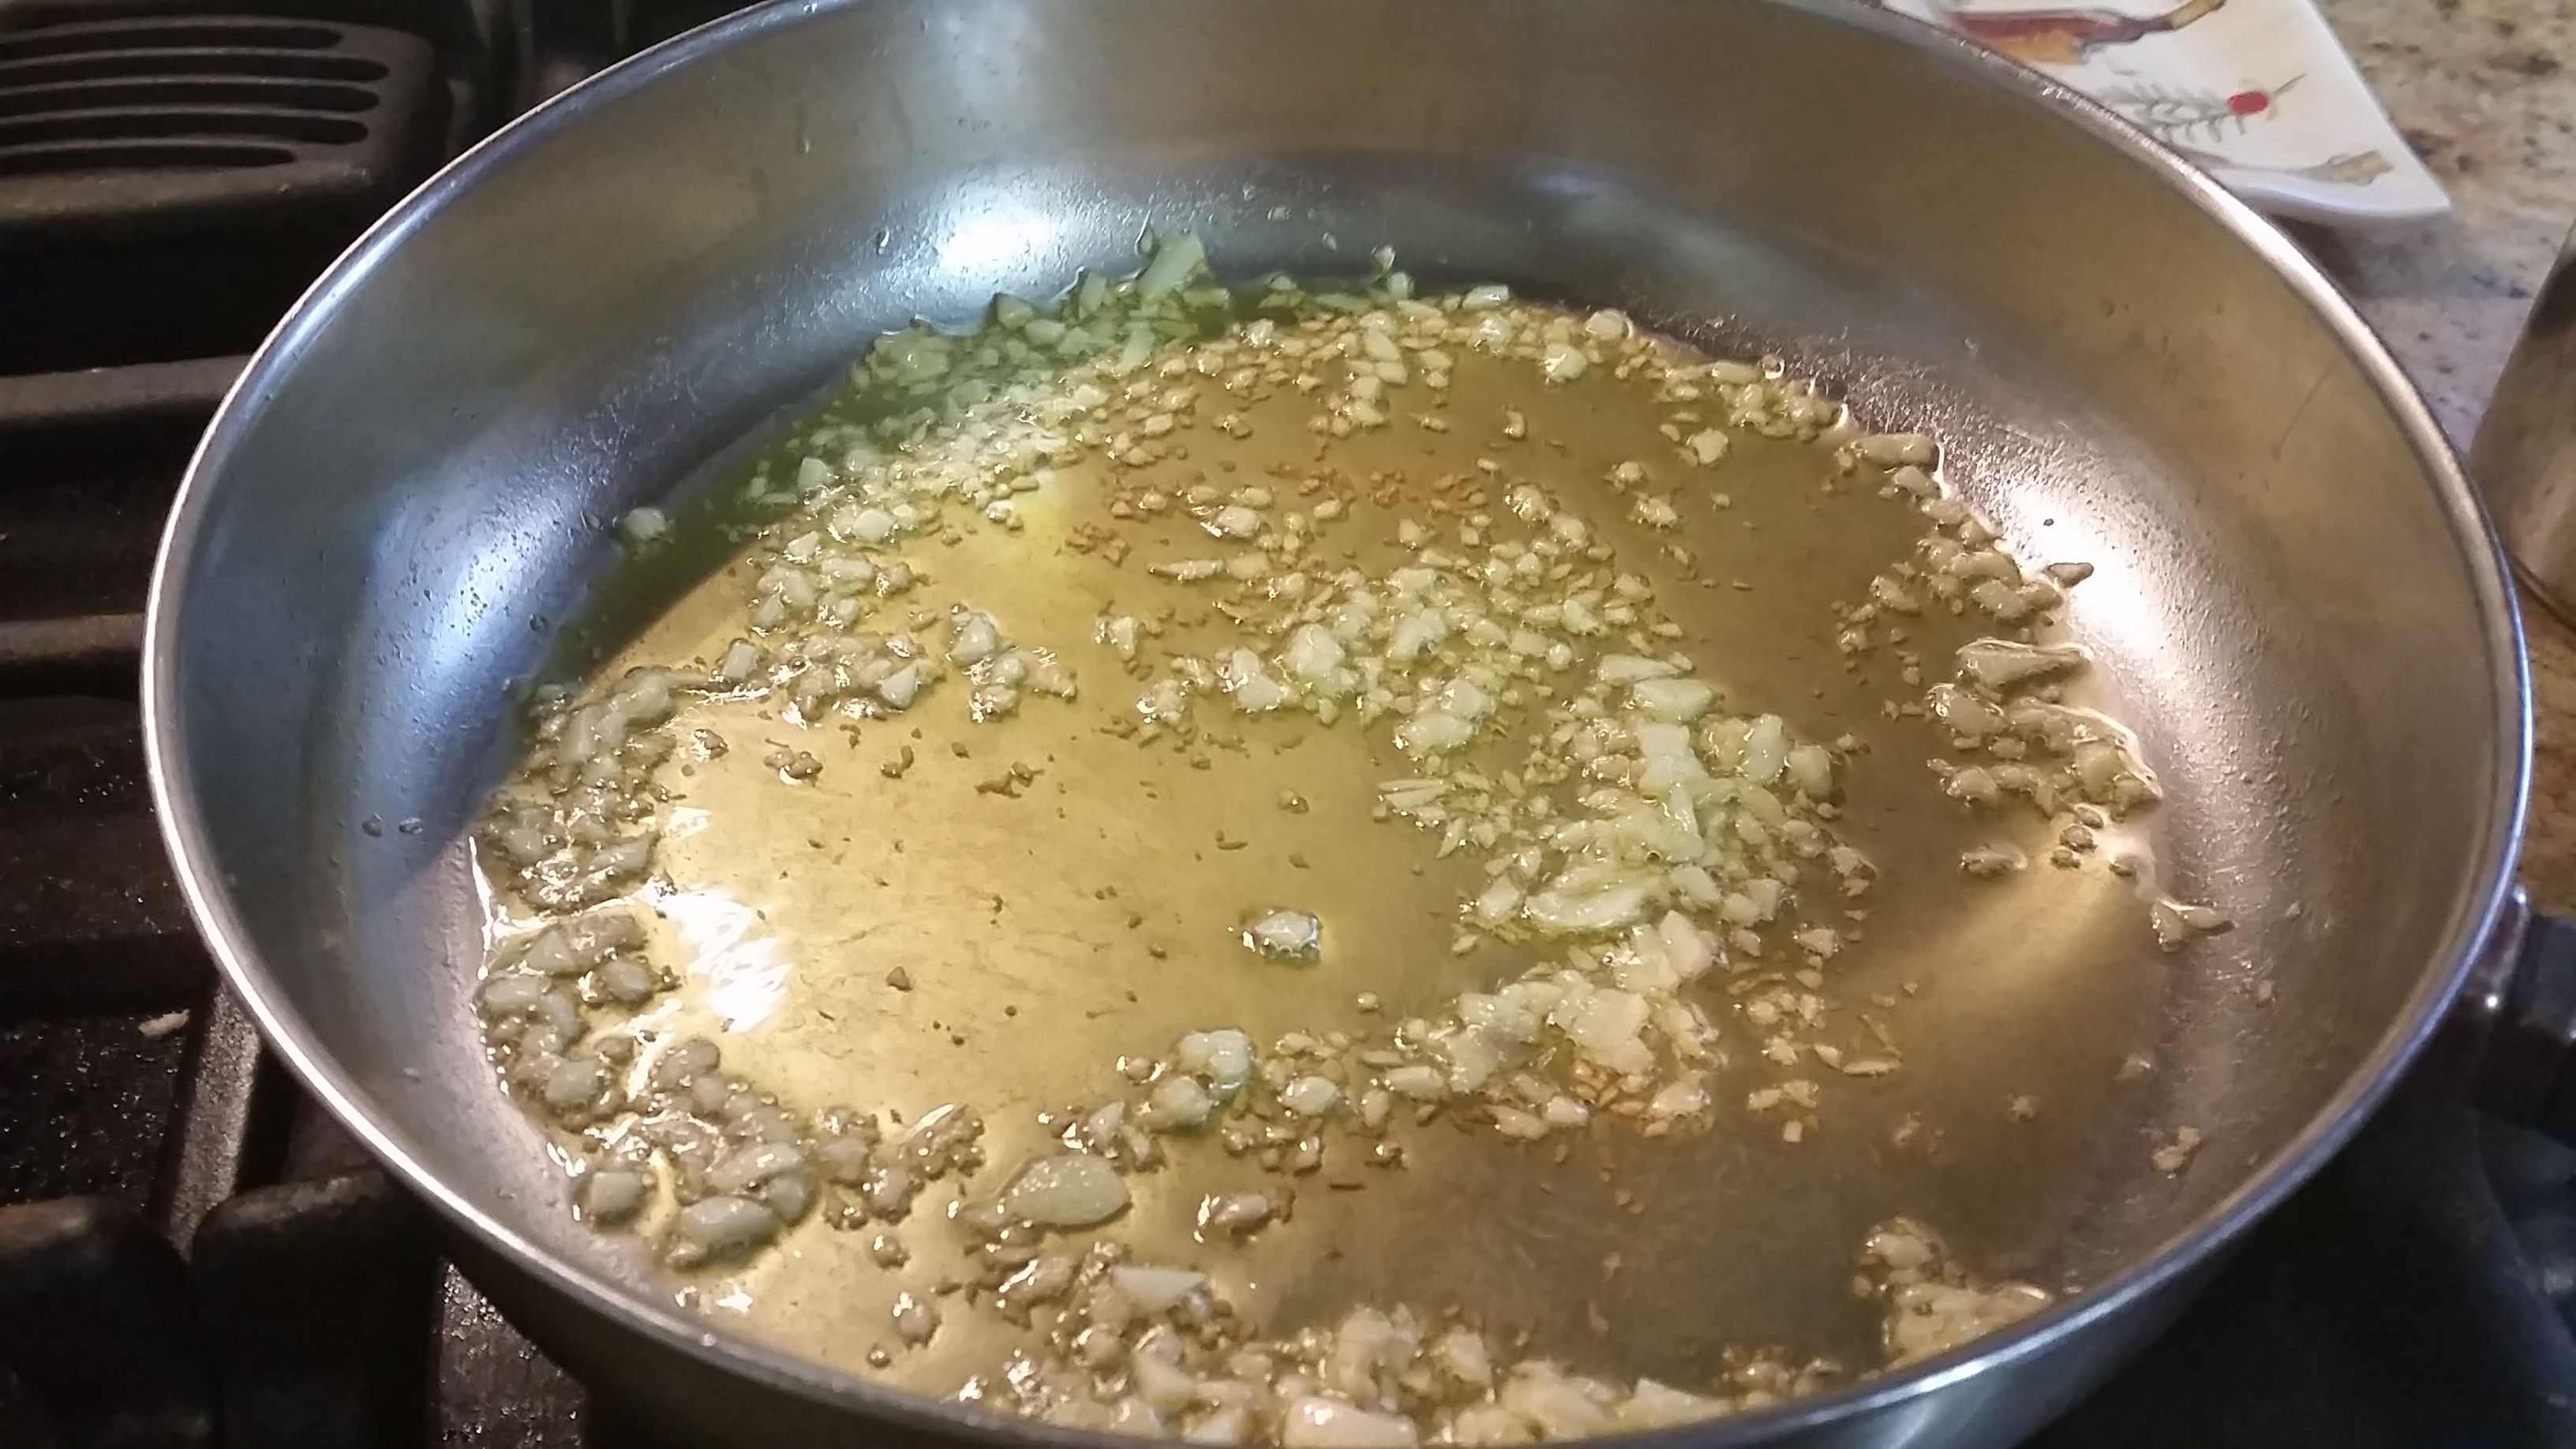
\includegraphics[width=0.5\textwidth]{stuffed_mushrooms/20150728_142924.jpg}%
		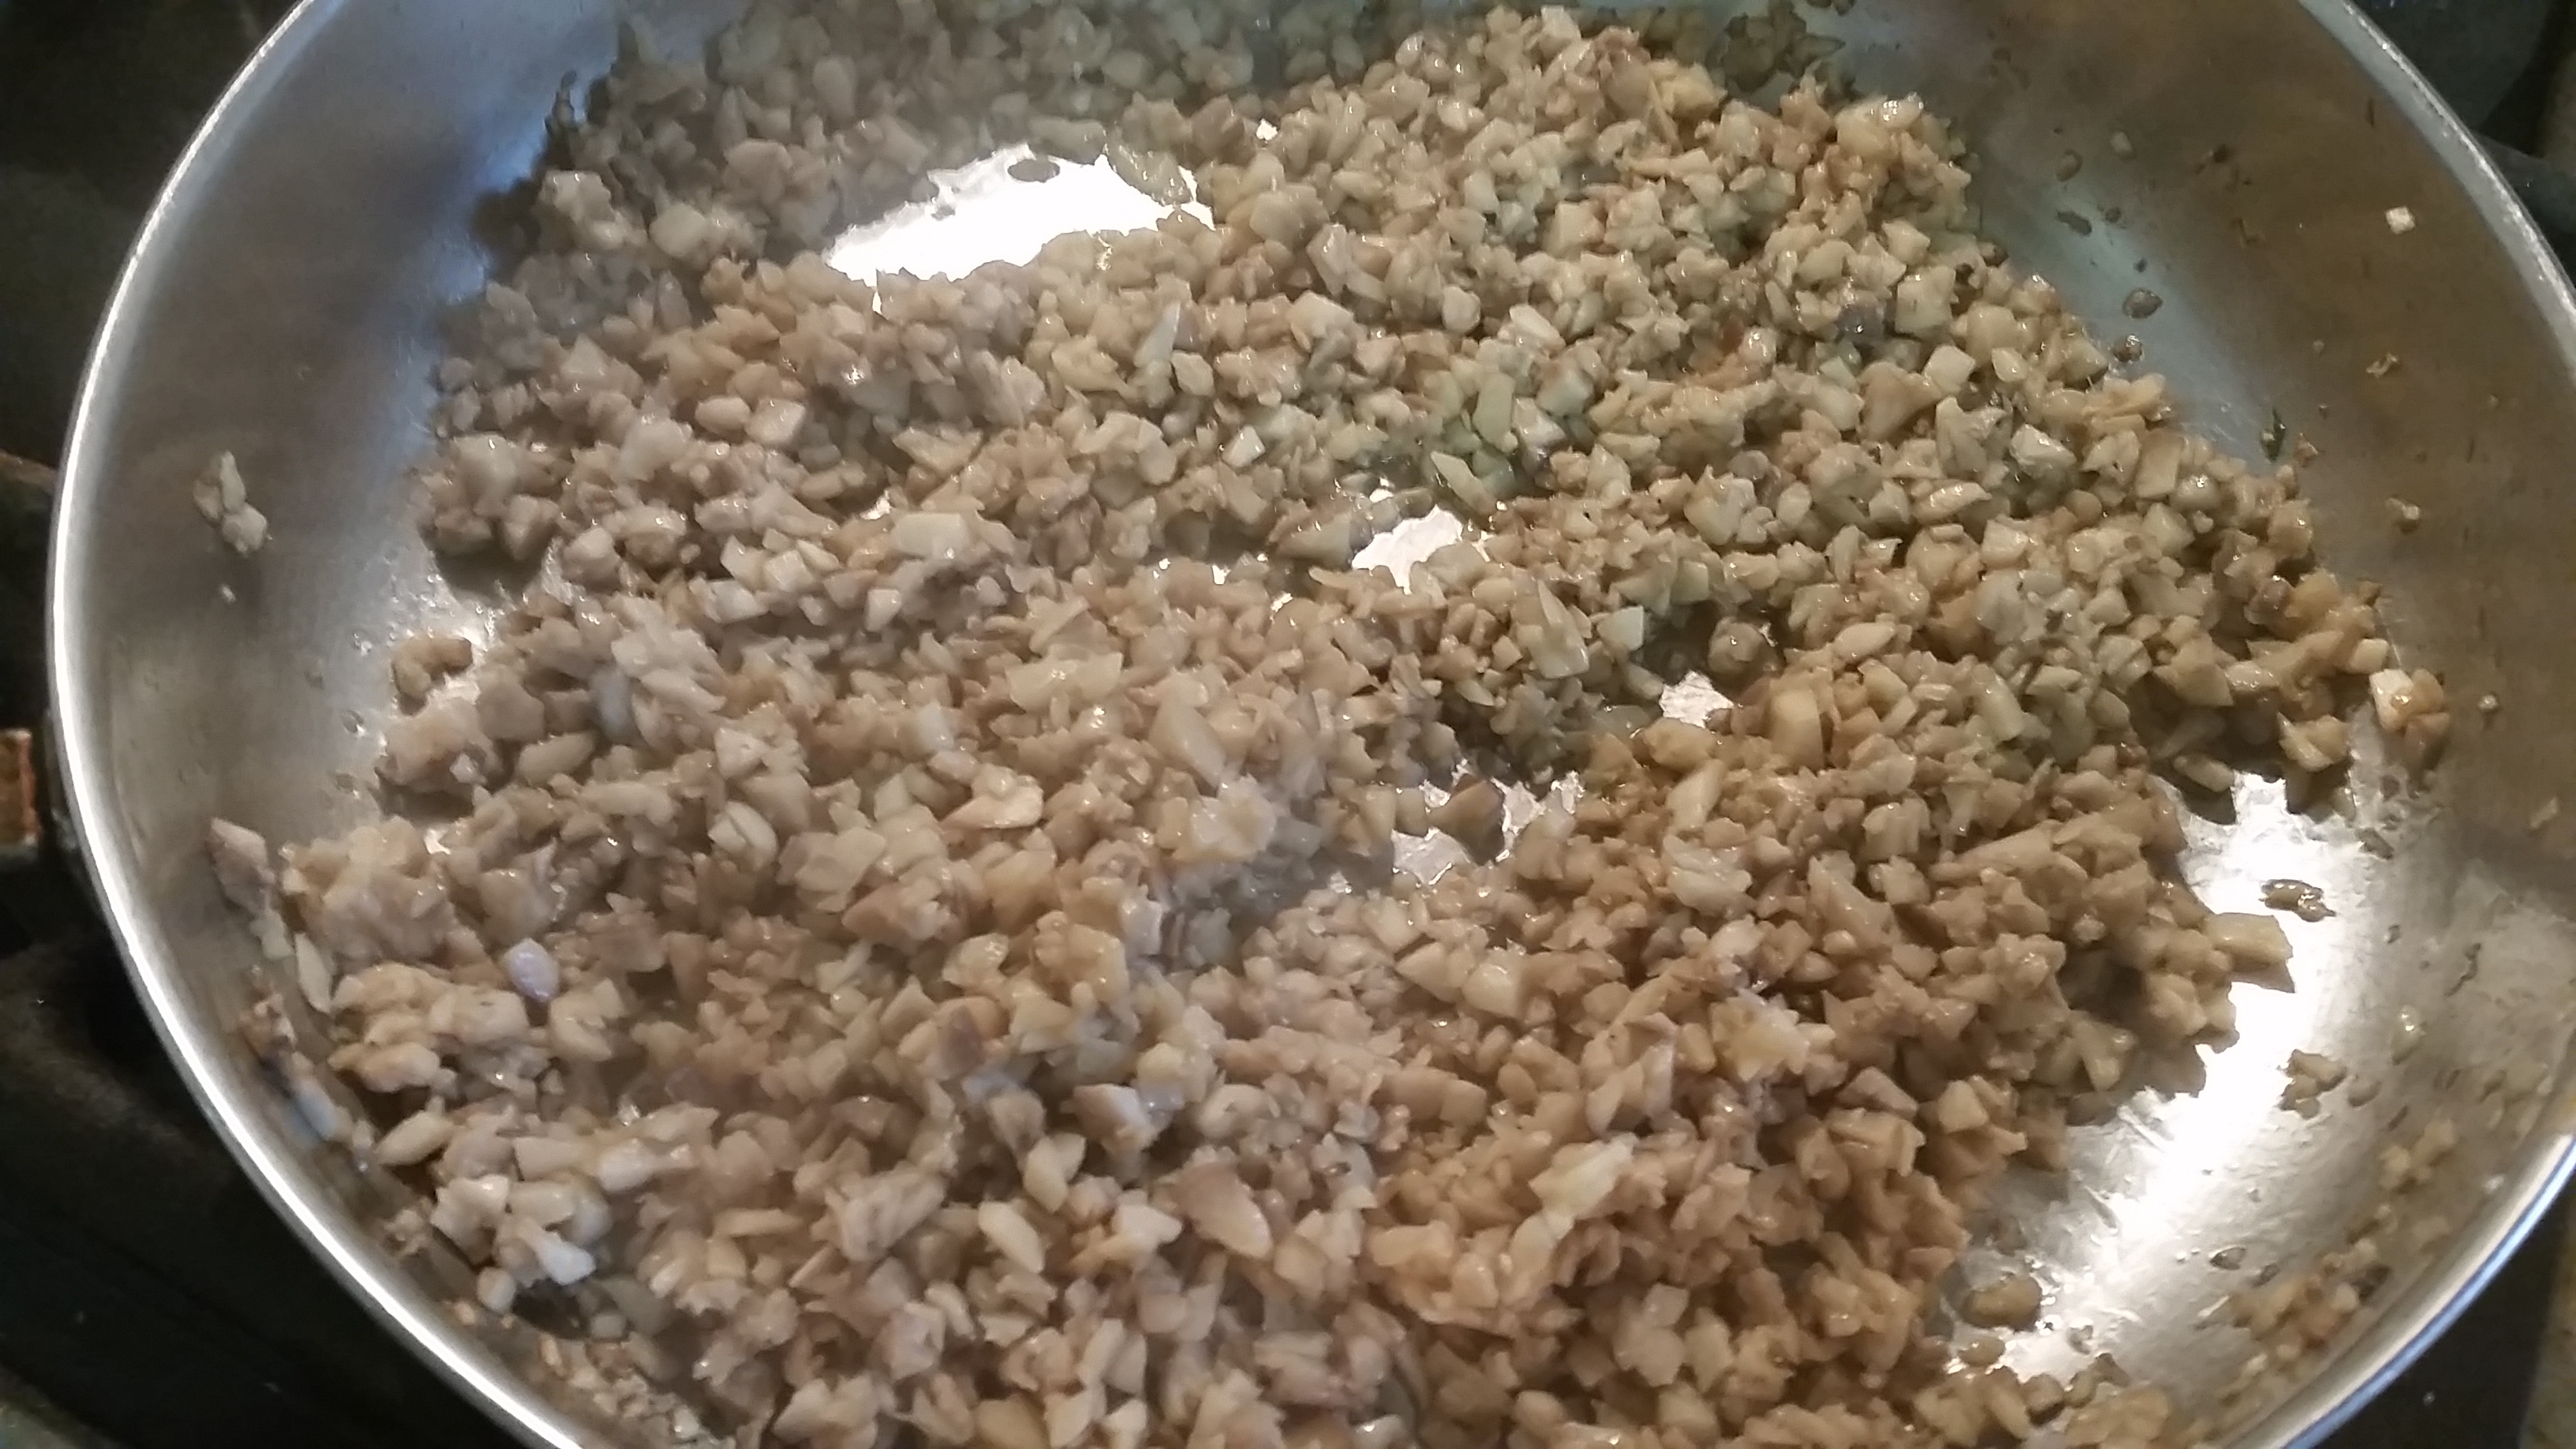
\includegraphics[width=0.5\textwidth]{stuffed_mushrooms/20150728_143650.jpg}

		\step In a large saute pan, add enough olive oil to give a significant coating to the bottom of the pan and heat until it shimmers (this will look like little waves passing through it.) Add in the garlic and cook until slightly brown.

		\step Throw in the mushroom stems and cook until the stems are soft and brown. Don't worry if the oil looks like it is far too much to fry so little in. The breadcrumbs will soak it up easily.

		\step Preheat your oven to \SI{350}{\fahrenheit} (\SI{180}{\celsius}).

		\vspace{1em}

		\step Once the mushrooms and garlic are cooked, add in the breadcrumbs, cheese, and parsley. Here is your chance to adjust. If there isn't enough oil to wet all the breadcrumbs, add more. If the breadcrumbs didn’t soak up all the oil, add more breadcrumbs. Add more cheese, or parsley, or any other spices you would like at this point and keep tasting the filling until it is just right. It won't change much in baking. The stuffing should be wet enough that it holds together but only just.

		\step In a roasting pan or two, lay out all of the caps and stuff them generously. There is usually left over stuffing when I make these, but if it seems like your using too much too quickly after the first few add some more oil and breadcrumbs to your stuffing and mix it around. In my family, the left over stuffing somehow disappears during the rest of the cooking process.

		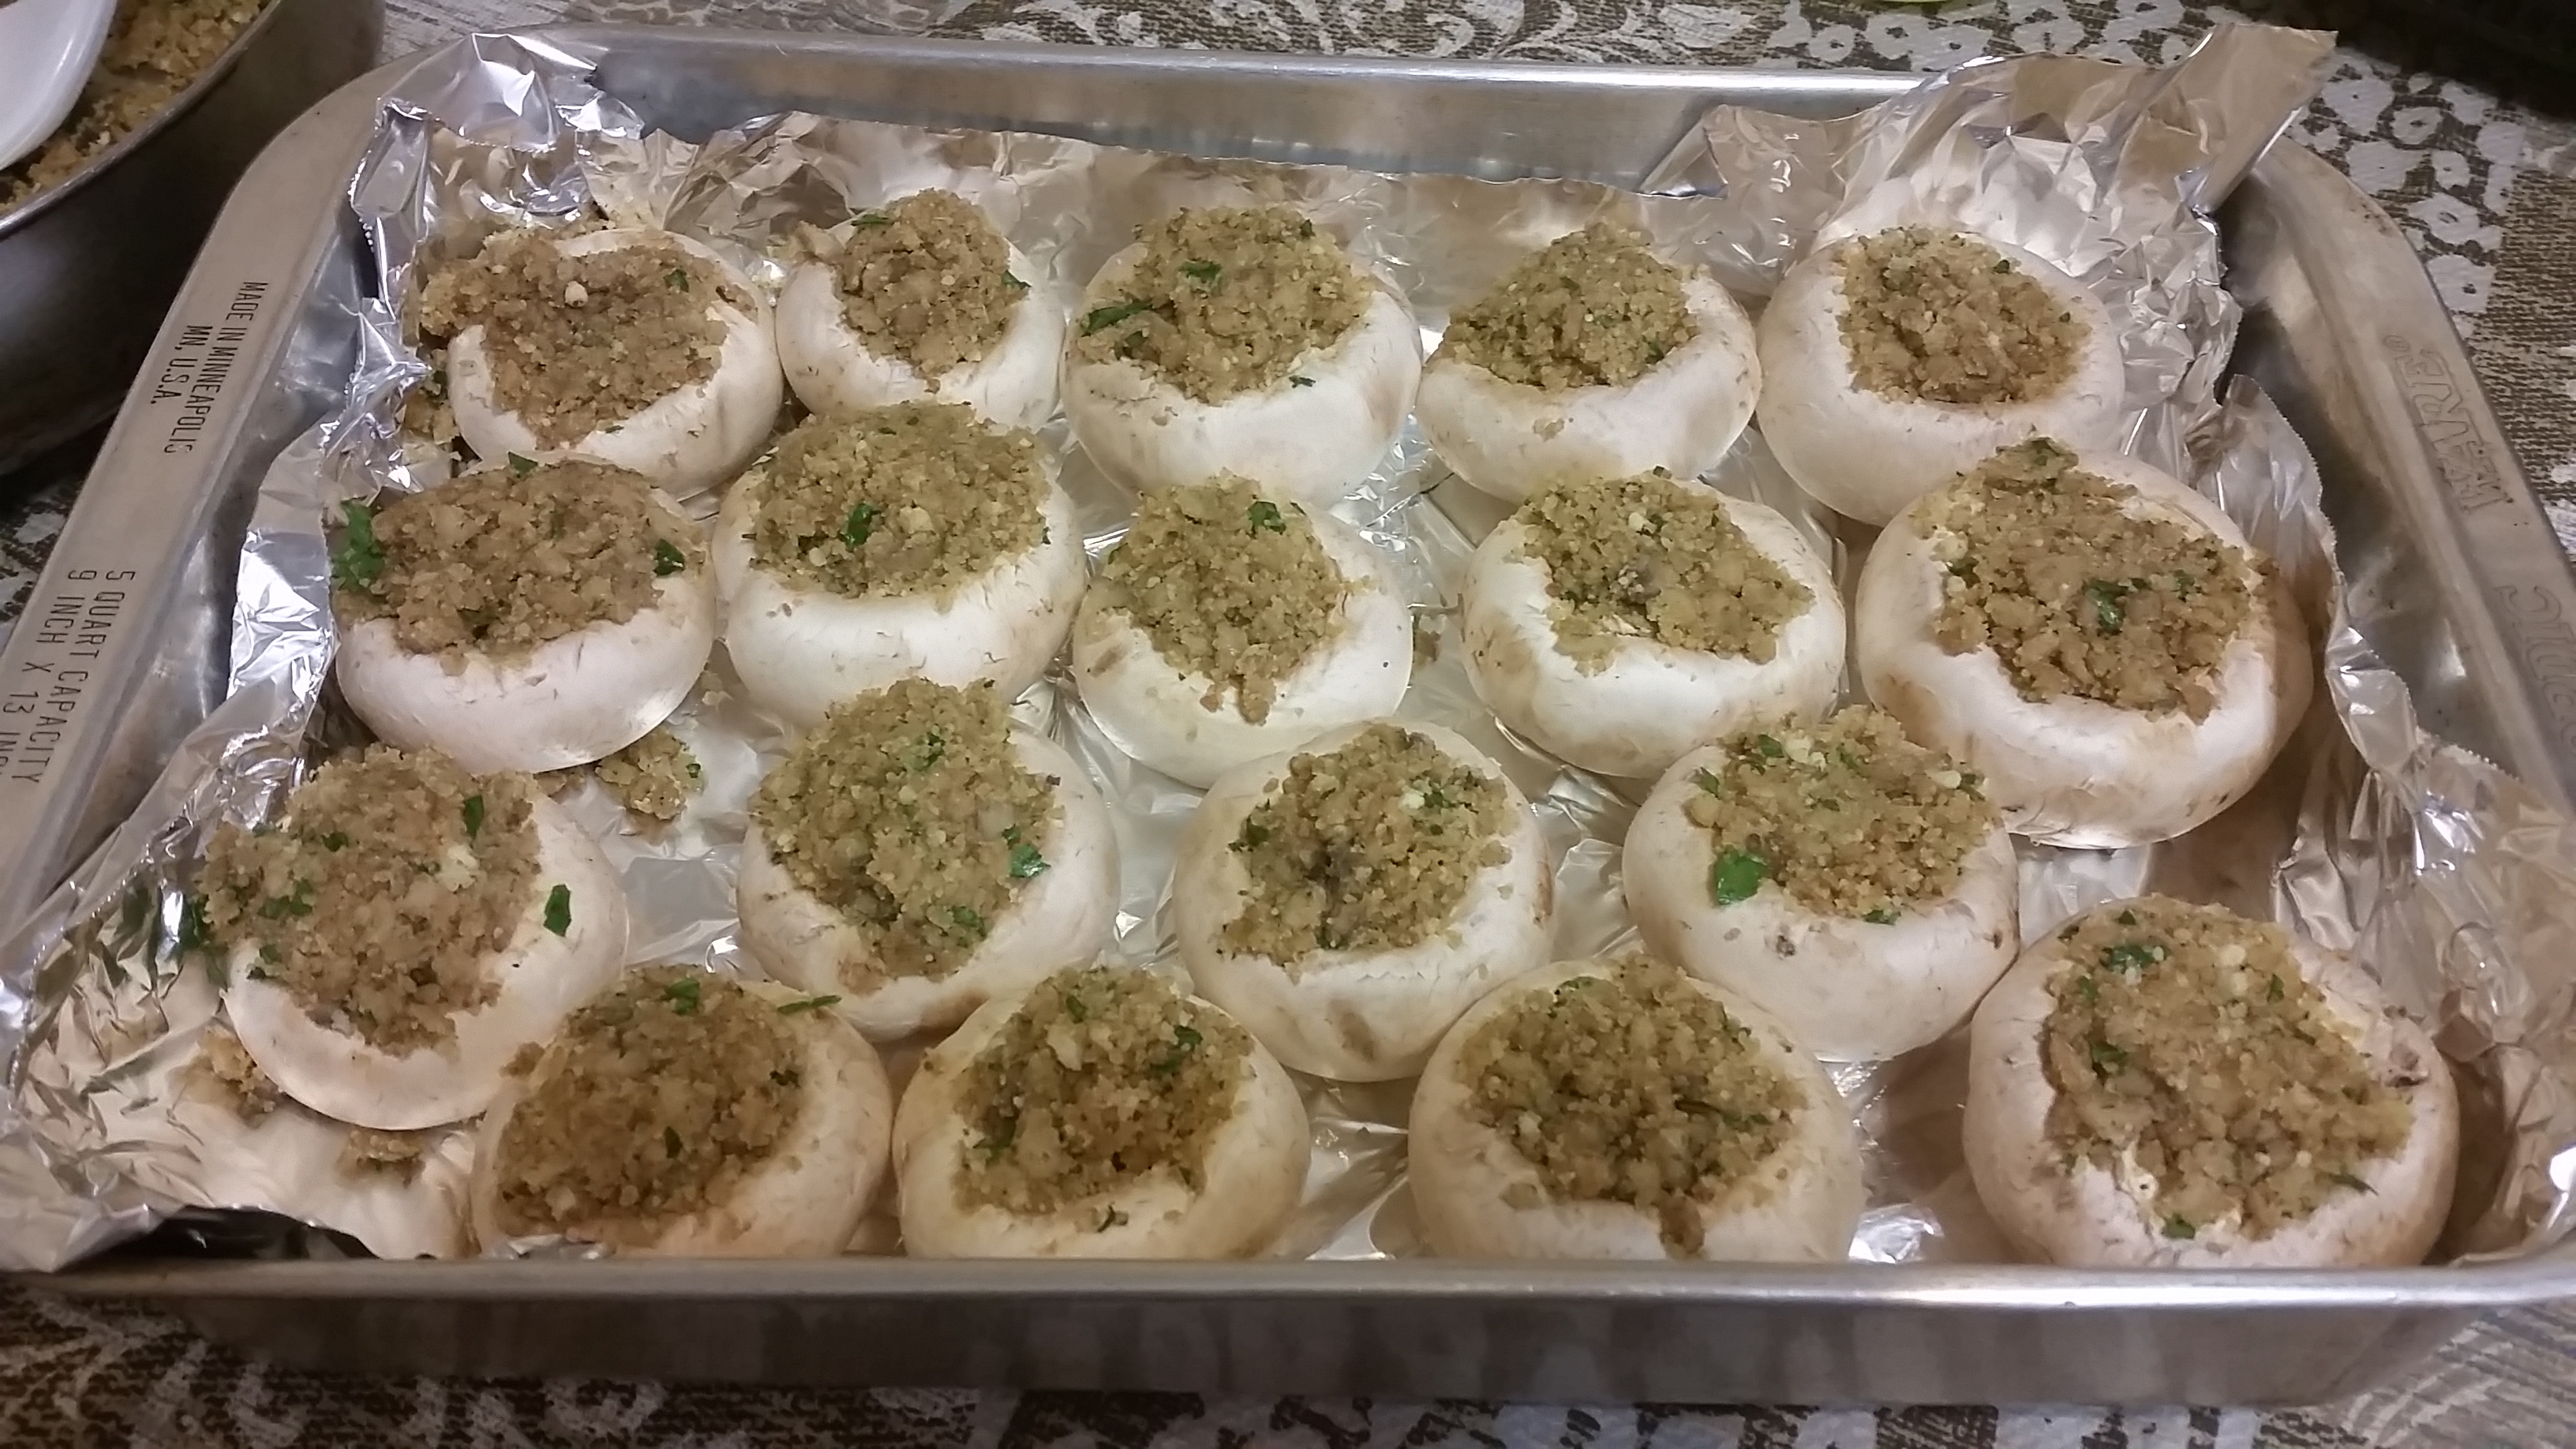
\includegraphics[width=0.5\textwidth]{stuffed_mushrooms/20150728_145435.jpg}%
		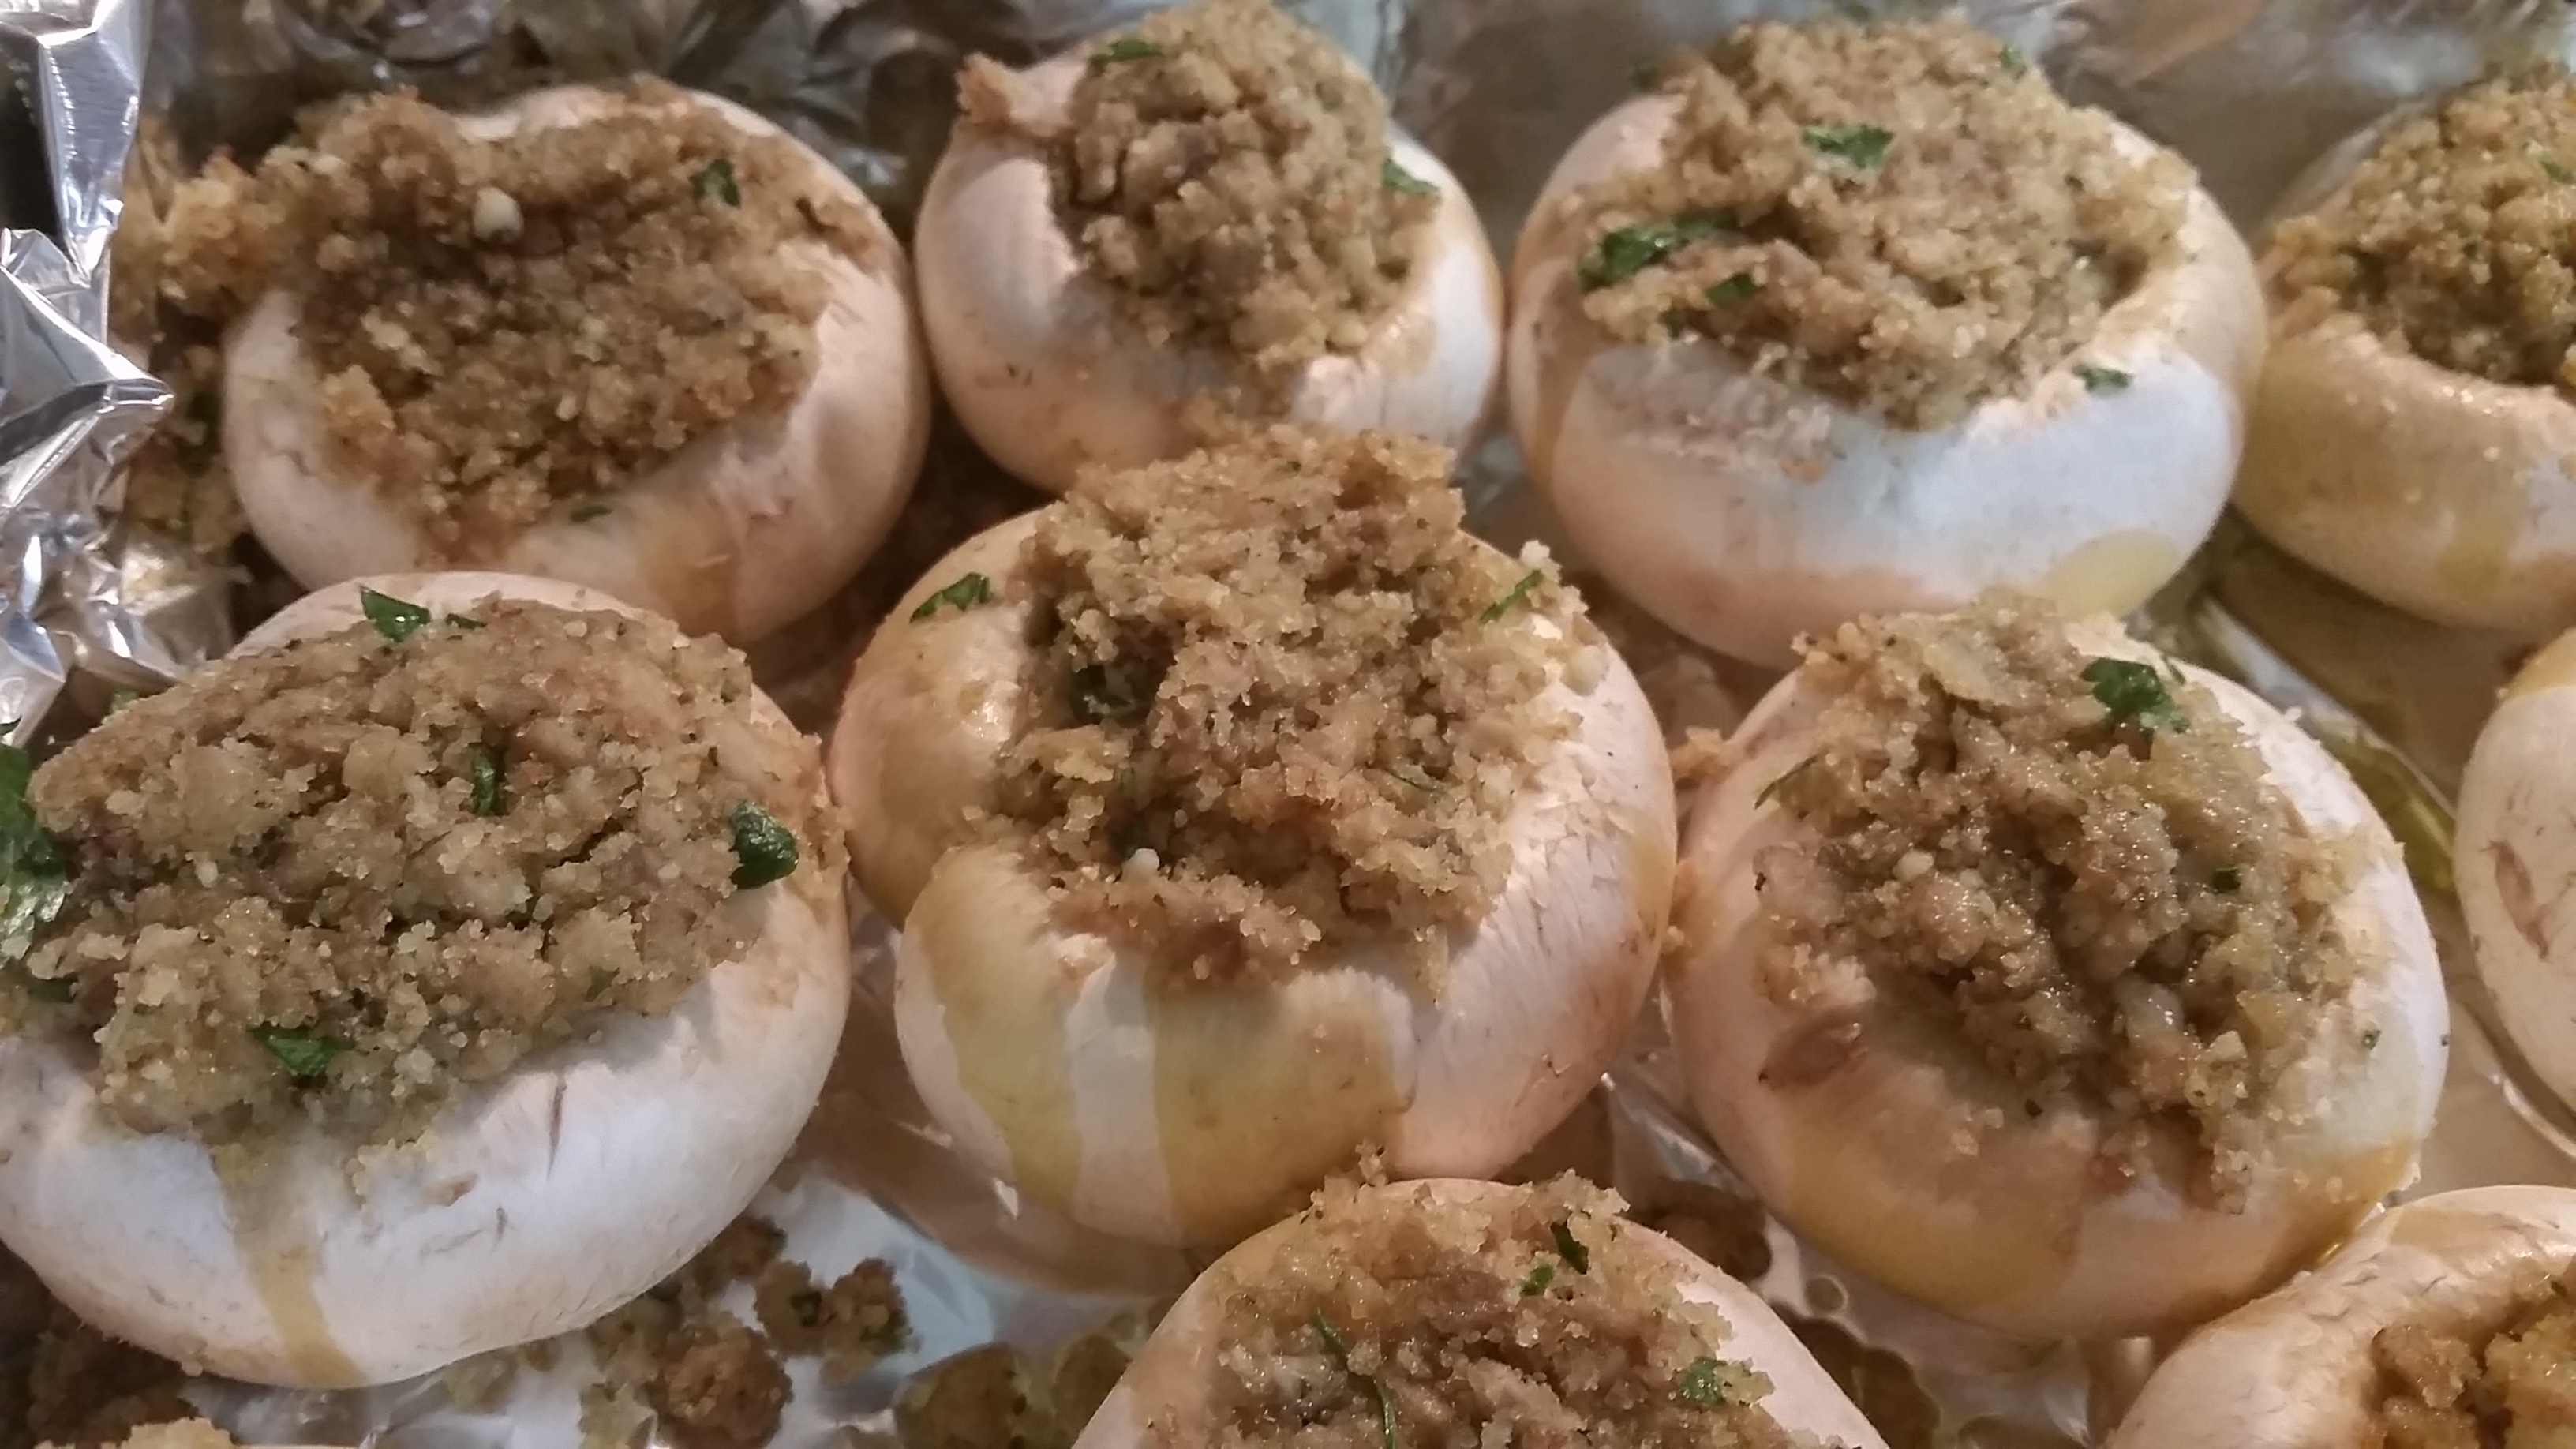
\includegraphics[width=0.5\textwidth]{stuffed_mushrooms/20150728_145858.jpg}

		\step After all of the caps are stuffed, drizzle some of the remaining oil over them (or water if you are looking to cut down on fat.) Stick them in the oven and let them cook for \SIrange{30}{35}{\minute} or until a toothpick slides through the flesh of the biggest mushroom cap with no resistance.

		\step Serve immediately or place in the fridge. They will keep for several days if stored in an air tight container, but are best eaten within one or two days. Reheat before serving, though sneaking a couple cold out of the fridge is still delicious.
	}

\end{recipe}